\documentclass[
11pt, %The default document font size, options: 10pt, 11pt, 12pt
]{charter} 

\usepackage{pgfgantt}
\usepackage{graphicx}
\usepackage{colortbl}
\usepackage{xcolor}
\usepackage{float}
\usepackage{tikz}
\usepackage{pdflscape}

% El títulos de la memoria, se usa en la carátula y se puede usar el cualquier lugar del documento con el comando \ttitle
\titulo{Beneficio en el uso de datos privados del buró frente al uso de datos públicos del BCRA para scoring de riesgo crediticio} 


% Nombre del posgrado, se usa en la carátula y se puede usar el cualquier lugar del documento con el comando \degreename
\posgrado{Carrera de Especialización en Inteligencia Artificial}


% Tu nombre, se puede usar el cualquier lugar del documento con el comando \authorname
% IMPORTANTE: no omitir titulaciones ni tildación en los nombres, también se recomienda escribir los nombres completos (tal cual los tienen en su documento)
\autor{Ing. Andrés Montes de Oca}

% El nombre del director y co-director, se puede usar el cualquier lugar del documento con el comando \supname y \cosupname y \pertesupname y \pertecosupname
\director{Paz Llamosas}
\pertenenciaDirector{UTN} 
\codirector{Lic. Mg. Erica Grinberg} % para que aparezca en la portada se debe descomentar la opción codirector en los parámetros de documentclass
\pertenenciaCoDirector{UNTREF}

% Nombre del cliente, quien va a aprobar los resultados del proyecto, se puede usar con el comando \clientename y \empclientename
\cliente{Nombre del cliente}
\empresaCliente{Empresa del cliente}
 
\fechaINICIO{27 de abril de 2026}		%Fecha de inicio de la cursada de GdP \fechaInicioName
\fechaFINALPlan{19 de junio de 2026} 	%Fecha de final de cursada de GdP
\fechaFINALTrabajo{diciembre de 2026}	%Fecha de defensa pública del trabajo final


\begin{document}

\maketitle
\thispagestyle{empty}
\pagebreak


\thispagestyle{empty}
{\setlength{\parskip}{0pt}
\tableofcontents{}
}
\pagebreak


\section*{Registros de cambios}
\label{sec:registro}

\begin{table}[ht]
\label{tab:registro}
\centering
\begin{tabularx}{\linewidth}{@{}|c|X|c|@{}}
\hline
\rowcolor[HTML]{C0C0C0} 
Revisión & \multicolumn{1}{c|}{\cellcolor[HTML]{C0C0C0}Detalles de los cambios realizados} & Fecha      \\ \hline
0      & Creación del documento.                                 & \fechaInicioName \\ \hline
1      & Se completa hasta el punto 5 inclusive.                 & 10 de mayo de 2026 \\ \hline
2      & Se completa hasta el punto 9 inclusive.				  & 17 de mayo de 2026 \\ \hline
3	   & Se completa hasta el punto 12 inclusive.       & 22 de mayo de 2026 \\ \hline
%  Se puede agregar algo más \newline
%  En distintas líneas \newline
%  Así                                                    & {día} de {mes} de 202X \\ \hline
%3      & Se completa hasta el punto 12 inclusive                & {día} de {mes} de 202X \\ \hline
%4      & Se completa el plan                                 & {día} de {mes} de 202X \\ \hline

% Si hay más correcciones pasada la versión 4 también se deben especificar acá

\end{tabularx}
\end{table}

\pagebreak



\section*{Acta de constitución del proyecto}
\label{sec:acta}

\begin{flushright}
Buenos Aires, \fechaInicioName
\end{flushright}

\vspace{2cm}

Por medio de la presente se acuerda con el \authorname\hspace{1px} que su Trabajo Final de la \degreename\hspace{1px} se titulará ``\ttitle'' y consistirá en {evaluar la mejora en la predicción de riesgo crediticio al integrar datos de un buró privado frente al uso exclusivo de datos públicos del BCRA}. El trabajo tendrá un presupuesto preliminar estimado de {620} horas y un costo estimado de {\$ 76,763,360}, con fecha de inicio el \fechaInicioName\hspace{1px} y fecha de presentación pública en \fechaFinalName.

Se adjunta a esta acta la planificación inicial.

\vfill

% Esta parte se construye sola con la información que hayan cargado en el preámbulo del documento y no debe modificarla
\begin{table}[ht]
\centering
\begin{tabular}{ccc}
\begin{tabular}[c]{@{}c@{}}Dr. Ing. Ariel Lutenberg \\ Director posgrado FIUBA\end{tabular} & \hspace{2cm} & \begin{tabular}[c]{@{}c@{}}\clientename \\ \empclientename \end{tabular} \vspace{2.5cm} \\ 
\multicolumn{3}{c}{\begin{tabular}[c]{@{}c@{}} \supname \\ Director del Trabajo Final\end{tabular}} \vspace{2.5cm} \\
\end{tabular}
\end{table}




\section{1. Descripción técnica-conceptual del proyecto a realizar}
\label{sec:descripcion}

En el ámbito de la gestión del riesgo crediticio, la correcta estimación de la probabilidad de default es un pilar fundamental para la sostenibilidad financiera. Tradicionalmente, los modelos de scoring han dependido de datos públicos y transaccionales, como los provistos por la Central de Deudores del Banco Central de la República Argentina (BCRA). Si bien estos datos ofrecen un panorama regulatorio del endeudamiento, suelen carecer de la granularidad necesaria sobre el comportamiento histórico de pago en el ecosistema financiero no regulado y comercial.

El problema analítico central radica en determinar y cuantificar empíricamente si la integración de datos de comportamiento provenientes de burós de crédito privados aporta un valor predictivo incremental que justifique su costo de adquisición. El estado del arte en modelado predictivo indica que la utilización de algoritmos de ensamble (tales como Gradient Boosting o Random Forest) permite maximizar la capacidad de discriminación al capturar interacciones no lineales complejas entre estas múltiples fuentes de datos estructurados.

La propuesta de valor de este proyecto consiste en desarrollar, entrenar y evaluar rigurosamente modelos de machine learning para la clasificación de riesgo, contrastando el desempeño de un modelo base (entrenado exclusivamente con variables públicas del BCRA) contra un modelo extendido (enriquecido con features privadas del buró). La validación metodológica de esta hipótesis se centrará en la evaluación del poder de separación poblacional en distintos segmentos de riesgo, priorizando métricas de discriminación avanzadas, fundamentalmente la mejora porcentual del estadístico Kolmogorov-Smirnov (KS) máximo.

\begin{figure}[htpb]
\centering 
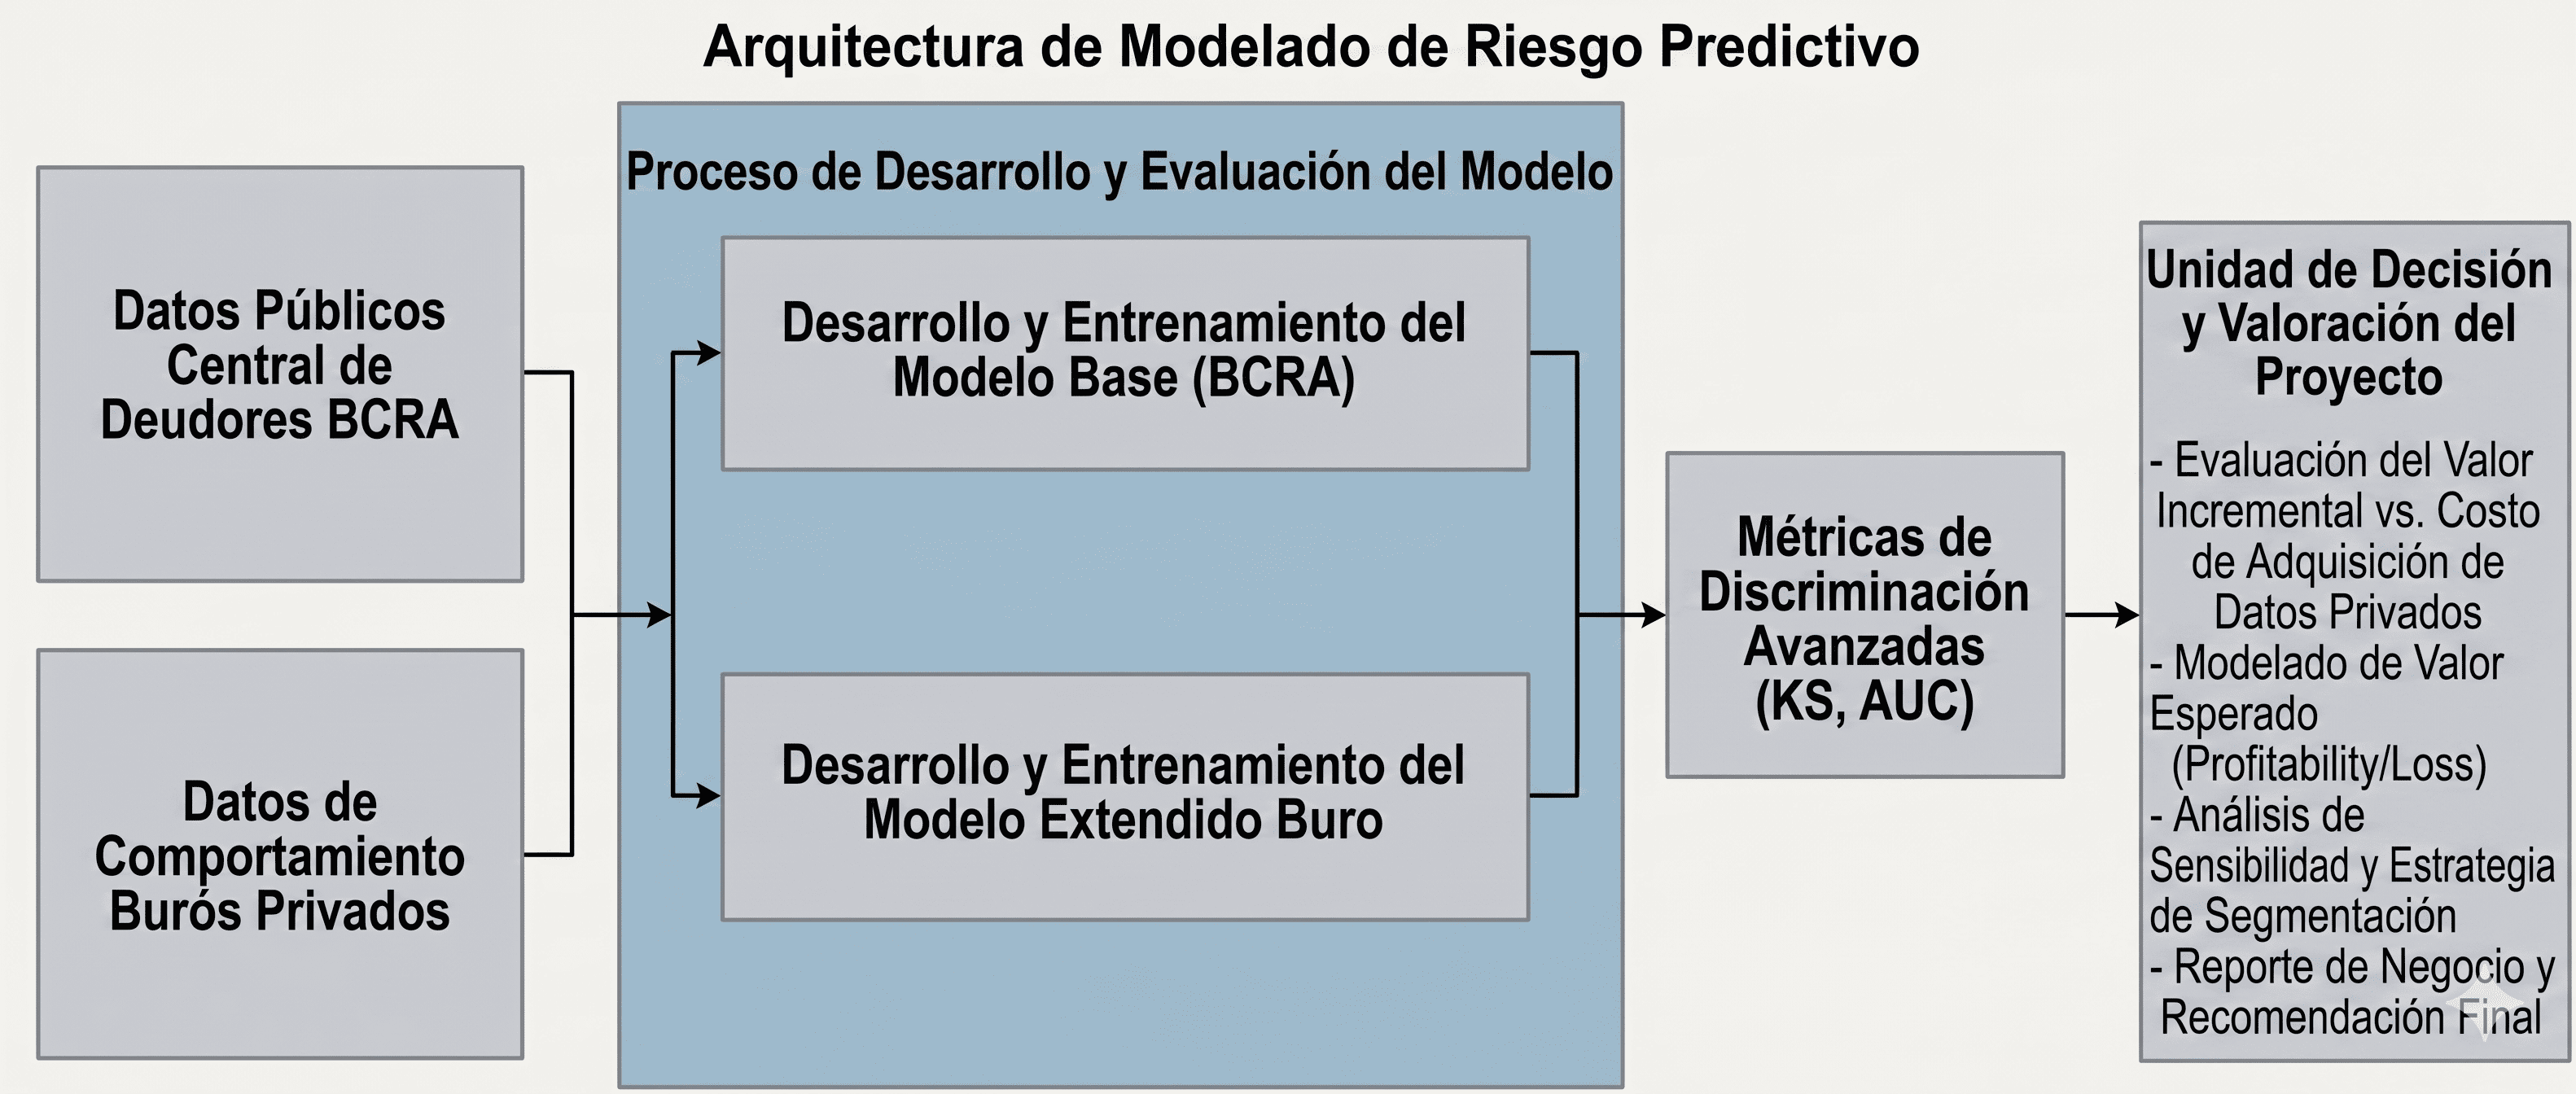
\includegraphics[width=.95\textwidth]{./Figuras/Modelado.png}
\caption{Diagrama en bloques del sistema.}
\label{fig:diagBloques}
\end{figure}

\vspace{25px}

\section{2. Identificación y análisis de los interesados}
\label{sec:interesados}

En el desarrollo de modelos predictivos de riesgo crediticio, la correcta identificación de los interesados resulta imperativa para garantizar que los requerimientos analíticos y las métricas de \textit{performance} se ajusten a la necesidad real del negocio. La propuesta de valor empírica de este proyecto exige una validación rigurosa por parte de los actores clave para contrastar el valor de la información de comportamiento del buró privado frente a los scores genéricos.

\begin{table}[ht]
\caption{Identificación de los interesados}
\label{tab:interesados}
\begin{tabularx}{\linewidth}{@{}|l|X|X|l|@{}}
\hline
\rowcolor[HTML]{C0C0C0}
Rol & Nombre y Apellido & Organización & Puesto \\ \hline
Cliente & John Doe & Nueva Financiera & Responsable de Riesgo \\ \hline
Responsable & \authorname & FIUBA & Alumno \\ \hline
Orientador & \supname & \pertesupname & Director del Trabajo Final \\ \hline
Opositores & Pepe Nova & Nueva Financiera & Responsable de Finanzas \\ \hline
\end{tabularx}
\end{table}

A continuación, se detallan las principales características y expectativas metodológicas de cada interesado clave con relación al proyecto:

\begin{itemize}
\item \textbf{Cliente (John Doe):} Es el responsable directo que aprobará los resultados y validará el entregable final. Su evaluación se centrará empíricamente en corroborar si el enriquecimiento algorítmico con datos privados aporta un incremento estadísticamente significativo en la métrica del estadístico Kolmogorov-Smirnov (KS), justificando su viabilidad comercial frente a modelos puramente transaccionales.
\item \textbf{Responsable (\authorname):} Ejerce la autoridad operativa y analítica para gestionar el ciclo de vida del proyecto, abarcando desde la recolección e imputación de variables, hasta la calibración de los hiperparámetros de los algoritmos de ensamble y la contrastación rigurosa de las distribuciones poblacionales.
\item \textbf{Orientador (\supname):} Como experto técnico, supervisará el rigor académico de la experimentación y el diseño algorítmico. Se encargará de asegurar la correcta partición de conjuntos de validación, previniendo sesgos o el sobreajuste (\textit{overfitting}) en la comparación de las fuentes públicas y privadas.
\item \textbf{Cliente Opositor (Pepe Nova):} Representan al grupo interno de la entidad cliente que prioriza la reducción de costos operativos a corto plazo. Su oposición radica en considerar el proyecto financieramente oneroso, prefiriendo la utilización exclusiva de datos públicos del BCRA (CENDEU) por ser económicamente más viable, aun asumiendo un detrimento en la \textit{performance} predictiva. El rigor de esta investigación deberá refutar empíricamente su postura, demostrando que la mejora en la capacidad de discriminación (medida a través del KS) compensa holgadamente el costo de adquisición de los datos de buró.
\end{itemize}

\section{3. Propósito del proyecto}
\label{sec:proposito}

Desarrollar y validar empíricamente un modelo predictivo de aprendizaje automático que cuantifique el valor analítico incremental de integrar datos de comportamiento provenientes de un buró de crédito privado frente a la utilización exclusiva de información pública transaccional del BCRA. Este esfuerzo metodológico busca optimizar las políticas de otorgamiento de crédito al maximizar la capacidad de discriminación poblacional, evaluada rigurosamente mediante el estadístico Kolmogorov-Smirnov (KS), proporcionando así la evidencia cuantitativa y objetiva necesaria para justificar económicamente la adquisición de fuentes de datos externas frente a las alternativas genéricas de bajo costo.

\section{4. Alcance del proyecto}
\label{sec:alcance}

El presente proyecto se circunscribe empíricamente al desarrollo, calibración y validación \textit{offline} de modelos predictivos de riesgo crediticio. El esfuerzo analítico se concentrará en cuantificar la mejora de la capacidad de discriminación poblacional, evaluada rigurosamente mediante el estadístico Kolmogorov-Smirnov (KS), al integrar fuentes del buró privado frente a los datos públicos del BCRA.

\textbf{El proyecto incluye taxativamente:}
\begin{itemize}
\item Extracción, depuración y análisis exploratorio exhaustivo de las bases de datos transaccionales públicas (CENDEU) y del buró de crédito privado.
\item Transformación de variables, imputación de valores faltantes e ingeniería de características (\textit{feature engineering}) orientada a capturar el comportamiento financiero.
\item Entrenamiento, optimización de hiperparámetros y validación cruzada utilizando distintos algoritmos de aprendizaje de maquina.
\item Evaluación metodológica y comparativa del desempeño predictivo entre el modelo base (datos públicos) y el modelo enriquecido (datos privados).
\item Estructuración de los métodos de transformación y modelos de forma tal que sean capaces de ser ejecutados en modalidad \textit{batch} sobre un conjunto de usuarios.
\end{itemize}

\textbf{El proyecto no incluye:}
\begin{itemize}
\item El despliegue o integración (\textit{deployment}) de los modelos algorítmicos en la arquitectura de servidores de producción de la entidad financiera.
\item El desarrollo de una interfaz gráfica de usuario (GUI) o cuadros de mando interactivos para el usuario final.
\item La ejecución del modelo predictivo de clasificación de riesgo en tiempo real (\textit{real-time scoring}).
\item La adquisición o integración de bases de datos de fuentes externas adicionales a las ya provistas para el estudio.
\end{itemize}


\section{5. Supuestos del proyecto}
\label{sec:supuestos}

Para el desarrollo del presente proyecto de investigación empírica se supone que:
\begin{itemize}
\item Se dispondrá de acceso irrestricto, oportuno y continuo a las bases de datos históricas (tanto transaccionales públicas del CENDEU como de comportamiento del buró privado), asumiendo que las mismas poseen la profundidad temporal necesaria para capturar la ciclicidad del riesgo crediticio.
\item Existe una relación matemática subyacente y capturable algorítmicamente entre las variables predictivas históricas seleccionadas y la probabilidad empírica de \textit{default} de los perfiles analizados.
\item Se contará con la infraestructura computacional adecuada (entornos de procesamiento distribuido o máquinas virtuales de alta capacidad) para entrenar, validar y optimizar los hiperparámetros de algoritmos de ensamble complejos sin enfrentar cuellos de botella de memoria.
\item El entorno macroeconómico y el marco normativo del BCRA mantendrán un nivel de estabilidad razonable durante el período de estudio, garantizando que alteraciones exógenas extremas no distorsionen la evaluación comparativa del estadístico Kolmogorov-Smirnov (KS).
\item Se dispondrá del tiempo estipulado en la planificación y la continuidad operativa del Responsable del proyecto para abarcar todas las fases metodológicas del ciclo de vida de los datos, desde la depuración hasta la evaluación final del poder de separación poblacional.
\end{itemize}

\section{6. Requerimientos}
\label{sec:requerimientos}

\begin{itemize}

    \item \textbf{Requerimientos funcionales}
    \begin{itemize}
        \item El sistema debe entrenar y evaluar modelos predictivos de riesgo crediticio experimentando con distintos algoritmos, aislando el rendimiento del modelo base (datos públicos del BCRA) respecto del modelo enriquecido (datos privados del buró).
        \item El sistema debe predecir una variable objetivo (\textit{target} o marca de incumplimiento) definida taxativamente como la ocurrencia de un atraso de pago superior a 90 días en el transcurso de los 12 meses posteriores al punto de observación.
        \item El sistema debe calcular y reportar el estadístico Kolmogorov-Smirnov (KS) como métrica central para evaluar la capacidad del modelo para separar y discriminar las funciones de distribución de dos poblaciones mutuamente excluyentes: los buenos pagadores y los malos pagadores.
        \item El cálculo de variables, la ingeniería de características (\textit{feature engineering}) y la predicción del modelo deben estructurarse para ser ejecutados en modalidad \textit{batch} sobre un conjunto dado de usuarios.
    \end{itemize}

    \item \textbf{Requerimientos de datos a utilizar}
    \begin{itemize}
        \item Los datos transaccionales extraídos del buró privado y del BCRA deben abarcar un período histórico definido estrictamente como los 60 meses hacia atrás desde el punto de observación, y procesarse en entornos que garanticen su anonimato y confidencialidad.
        \item Cada usuario debe pertenecer de manera mutuamente excluyente a los conjuntos de entrenamiento, validación o prueba para evitar sesgos analíticos y filtración de información (\textit{data leakage}).
        \item El conjunto de datos crediticios utilizado para entrenar los algoritmos no debe ser compartido públicamente bajo ninguna circunstancia, respetando el marco normativo vigente.
    \end{itemize}

    \item \textbf{Requerimientos Normativos}
    \begin{itemize}
        \item El tratamiento, almacenamiento y análisis de la data de comportamiento proveniente del buró privado y de la Central de Deudores del BCRA (CENDEU) debe cumplir estrictamente con la Ley 25.326 de Protección de Datos Personales, garantizando la total anonimización de las variables para evitar la exposición de datos sensibles y asegurar la confidencialidad.
    \end{itemize}

    \item \textbf{Requerimientos de Testing}
    \begin{itemize}
        \item El sistema algorítmico debe ser evaluado indefectiblemente mediante pruebas de validación fuera de muestra (\textit{out-of-sample}) y validación cruzada (\textit{cross-validation}) para certificar empíricamente la robustez del modelo y la generalización de los resultados.
        \item La evaluación del desempeño debe cuantificar objetivamente la mejora en el estadístico Kolmogorov-Smirnov (KS) máximo del modelo híbrido frente al modelo base evaluado en las particiones de prueba, demostrando rigurosamente la ausencia de sobreajuste (\textit{overfitting}).
    \end{itemize}

    \item \textbf{Requerimientos de documentación}
    \begin{itemize}
        \item Se debe redactar una memoria técnica detallando la optimización de hiperparámetros y el análisis exploratorio realizado sobre los conjuntos de datos.
        \item Se debe elaborar un informe que demuestre empíricamente el incremento porcentual del estadístico KS, justificando de manera cuantitativa la capacidad predictiva de los datos privados del buró frente al modelo base del BCRA.
        \item Se debe analizar y documentar la importancia predictiva de las variables independientes (\textit{feature importance}) para garantizar la explicabilidad y transparencia del \textit{scoring} crediticio.
    \end{itemize}

\end{itemize}

\section{7. Historias de usuarios (\textit{Product backlog})}
\label{sec:backlog}

Para la ponderación de las historias de usuario se utilizarán tres criterios, cada uno con tres niveles posibles de calificación:

\begin{itemize}

    \item \textbf{Dificultad}
    \begin{itemize}
        \item Baja: 1 punto
        \item Media: 3 puntos
        \item Alta: 5 puntos
    \end{itemize}

    \item \textbf{Complejidad}
    \begin{itemize}
        \item Baja: 2 puntos
        \item Media: 5 puntos
        \item Alta: 7 puntos
    \end{itemize}

    \item \textbf{Incertidumbre}
    \begin{itemize}
        \item Baja: 1 punto
        \item Media: 5 puntos
        \item Alta: 10 puntos
    \end{itemize}

\end{itemize}

El puntaje final de cada historia de usuario será calculado como el número de la secuencia de Fibonacci más próximo mayor o igual a la suma de las calificaciones en los 3 criterios. A continuación, se detallan las historias agrupadas analíticamente por rol:

\begin{itemize}

    \item \textbf{Rol: Científico de Datos}
    \begin{itemize}
        \item Como Científico de Datos quiero entrenar un modelo base con información pública del BCRA y un modelo enriquecido con información del buró privado para aislar y cuantificar el incremento del estadístico KS en la separación de buenos y malos pagadores. (5+7+5 = 17 $\rightarrow$ 21 puntos)

        \item Como Científico de Datos quiero ejecutar una validación cruzada en diferentes ventanas temporales (\textit{Out-of-Time validation}) para asegurar que la estabilidad de las métricas de separación poblacional se mantenga constante y no sufra volatilidad a causa del sobreajuste algorítmico. (3+7+5 = 15 $\rightarrow$ 21 puntos)
    \end{itemize}

    \item \textbf{Rol: Analista de Riesgos}
    \begin{itemize}
        \item Como Analista de Riesgos quiero comparar empíricamente la capacidad de discriminación de ambos modelos a través de todos los deciles de riesgo, validando la consistencia predictiva en toda la distribución poblacional para justificar cuantitativamente la adquisición de datos de comportamiento no regulado. (3+5+5 = 13 $\rightarrow$ 13 puntos)

        \item Como Analista de Riesgos quiero evaluar la importancia de las variables independientes (\textit{feature importance}) del modelo híbrido para comprender qué características del buró privado determinan el comportamiento crediticio y garantizar la interpretabilidad de la decisión algorítmica. (3+5+1 = 9 $\rightarrow$ 13 puntos)

        \item Como Analista de Riesgos quiero calcular el Índice de Estabilidad Poblacional (PSI) de las variables estructuradas del buró privado para garantizar que las distribuciones no sufran deriva de datos (\textit{Data Drift}) temporal frente a la muestra base, asegurando la robustez y vigencia del modelo. (3+5+1 = 9 $\rightarrow$ 13 puntos)
    \end{itemize}

    \item \textbf{Rol: Analista de Finanzas}
    \begin{itemize}
        \item Como Analista del Sector de Finanzas quiero evaluar las predicciones del modelo híbrido para aumentar la cantidad de usuarios aprobados manteniendo el mismo porcentaje de malos pagadores de la cartera actual (\textit{estrategia de swap-in}), demostrando así la viabilidad comercial y operativa de la información externa. (3+5+1 = 9 $\rightarrow$ 13 puntos)
    \end{itemize}

    \item \textbf{Rol: Gobernanza de Datos}
    \begin{itemize}
        \item Como Responsable del área de Gobernanza de Datos quiero validar los \textit{pipelines} de preprocesamiento de características transaccionales para asegurar la anonimización de la información privada, certificando el cumplimiento de la Ley 25.326 de Protección de Datos Personales. (1+2+5 = 8 $\rightarrow$ 8 puntos)
    \end{itemize}

\end{itemize}

\section{8. Entregables principales del proyecto}
\label{sec:entregables}

Los entregables principales del proyecto son:
\begin{itemize}
    \item Memoria técnica del Trabajo Final, documentando la fundamentación empírica, la ingeniería de características y la justificación matemática del incremento en el estadístico Kolmogorov-Smirnov (KS) entre el modelo base (BCRA) y el modelo híbrido, omitiendo cualquier exposición de datos sensibles.
    \item Informe ejecutivo orientado al Sector de Finanzas, detallando de forma clara y directa el beneficio comercial del proyecto. Este documento demostrará empíricamente cómo el uso de los datos del buró permite aumentar la cantidad de usuarios aprobados manteniendo constante el porcentaje de malos pagadores en la cartera.
    \item \textit{Jupyter Notebooks} y \textit{pipeline} de procesamiento de datos. El código fuente no será entregado bajo ningún formato; por políticas de confidencialidad, únicamente estará disponible de forma exclusiva en un repositorio institucional privado.
\end{itemize}

\section{9. Desglose del trabajo en tareas}
\label{sec:wbs}

A continuación se detalla la Estructura de Desglose del Trabajo (EDT/WBS), donde cada paquete de trabajo ha sido descompuesto en tareas técnicas de duración no mayor a 40 horas para garantizar un seguimiento riguroso. El esfuerzo total estimado para este proyecto de modelado predictivo es de 620 horas.

\begin{itemize}

    \item \textbf{Estudio de la temática y marco normativo (100 h)}
    \begin{itemize}
        \item Lectura de bibliografía sobre modelos de ensamble aplicados a \textit{scoring} crediticio (40 h).
        \item Relevamiento del marco normativo (Ley 25.326) y pautas de gobernanza de datos para el anonimato (20 h).
        \item Exploración documental de la estructura de diccionarios de variables del BCRA (CENDEU) y del buró privado (40 h).
    \end{itemize}

    \item \textbf{Definición de lineamientos del modelo (70 h)}
    \begin{itemize}
        \item Formulación metodológica para la evaluación de la separación poblacional y umbrales del estadístico KS (40 h).
        \item Validación y ajuste de la propuesta analítica y métricas de éxito con el Sector de Finanzas (30 h).
    \end{itemize}

    \item \textbf{Obtención y preprocesamiento de datos (140 h)}
    \begin{itemize}
        \item Desarrollo de la consulta estructurada para la extracción de la ventana de observación histórica de 60 meses (40 h).
        \item Integración de los datos tabulares públicos (BCRA) con los datos externos (buró privado) garantizando anonimato (40 h).
        \item Definición y etiquetado de la variable objetivo (\textit{target}): atraso mayor a 90 días en la ventana de desempeño de 12 meses (30 h).
        \item Limpieza exhaustiva de la muestra, tratamiento de valores nulos y filtrado de \textit{outliers} (30 h).
    \end{itemize}

    \item \textbf{Desarrollo algorítmico y evaluación (210 h)}
    \begin{itemize}
        \item Análisis exploratorio de datos (EDA) y cálculo de la divergencia de distribuciones (30 h).
        \item Ingeniería de características (\textit{feature engineering}) y selección iterativa de variables predictivas (40 h).
        \item Partición de la muestra y entrenamiento secuencial del modelo base y el modelo enriquecido (40 h).
        \item Cálculo del Índice de Estabilidad Poblacional (PSI) y evaluación del peso predictivo de variables (\textit{feature importance}) (30 h).
        \item Cálculo y análisis comparativo del incremento del estadístico Kolmogorov-Smirnov (KS) en todos los deciles de riesgo (40 h).
        \item Armado del \textit{pipeline} definitivo para la productivización \textit{batch} y estimación de viabilidad comercial (\textit{swap-in}) (30 h).
    \end{itemize}

    \item \textbf{Documentación y cierre del proyecto (100 h)}
    \begin{itemize}
        \item Redacción de la memoria técnica documentando la experimentación empírica (40 h).
        \item Elaboración del informe ejecutivo analítico orientado al área de presupuesto y finanzas (30 h).
        \item Preparación del material audiovisual y simulacro para la defensa pública del trabajo (30 h).
    \end{itemize}

\end{itemize}


\begin{landscape}

\begin{center}
{\large\bfseries 10. Diagrama de Activity on Node}
\end{center}

\vspace*{\fill}

\begin{center}
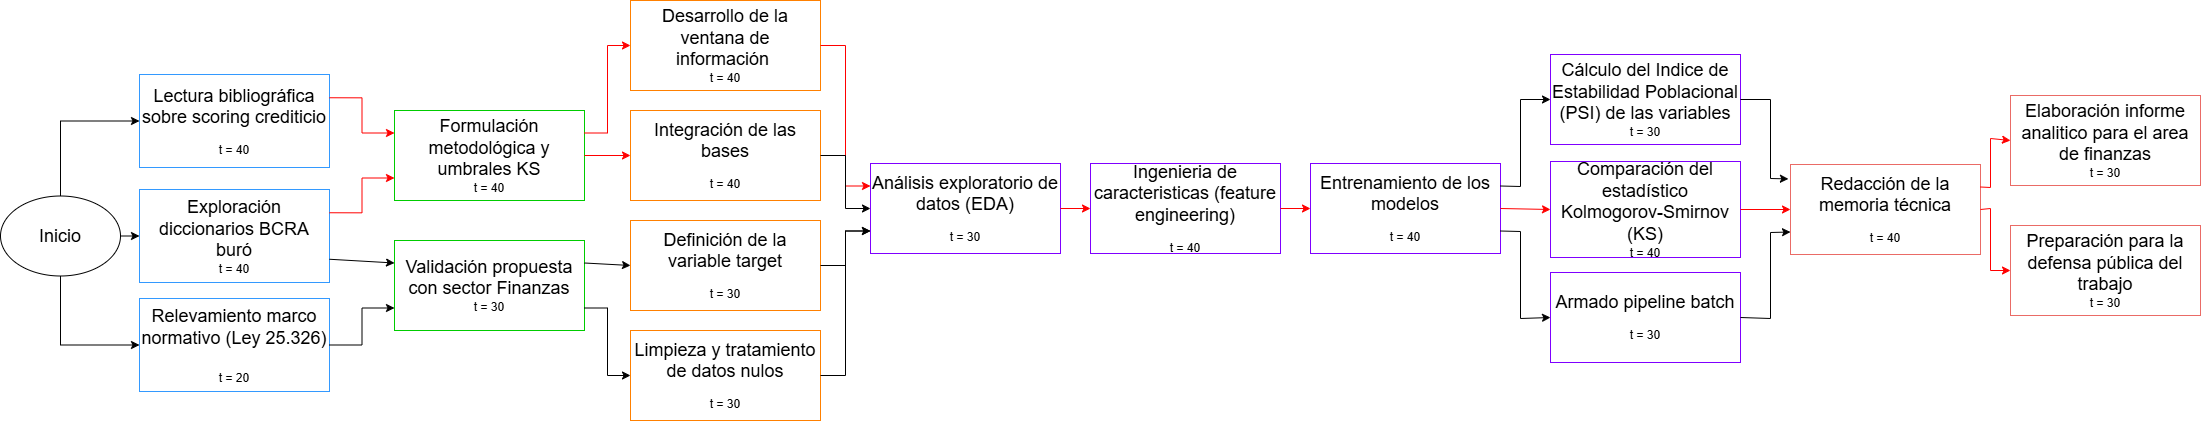
\includegraphics[width=0.88\linewidth, height=0.82\textheight, keepaspectratio]{./Figuras/AoN2.png}

\vspace{0.4cm}

{\small Figura 2. Diagrama Activity on Node con su camino cr\'itico en rojo.}
\end{center}

\vspace*{\fill}

\end{landscape}


\section{11. Diagrama de Gantt}
\label{sec:gantt}

Para el armado del diagrama de Gantt se tuvo en cuenta que la dedicaci\'{o}n al proyecto
ser\'{a} de lunes a viernes a raz\'{o}n de 5 horas por d\'{i}a. La fecha de inicio es el
27/04/2026 y la de finalizaci\'{o}n est\'{a} estimada para el 25/09/2026.
El esfuerzo total del proyecto es de 620 horas, distribuidas en cinco paquetes de trabajo.
Las barras en color azul corresponden a tareas t\'{e}cnicas, mientras que las barras
en color rojo oscuro representan las tareas no t\'{e}cnicas de documentaci\'{o}n y cierre.

\begin{center}
{\small \textbf{Cuadro 2.} Lista de tareas con fechas de inicio y fin.}

\vspace{0.2cm}
\scriptsize
\setlength{\tabcolsep}{4pt}
\begin{tabular}{|c|p{6.5cm}|c|c|c|c|c|}
\hline
\rowcolor[HTML]{C0C0C0}
\textbf{Id} & \textbf{Nombre} & \textbf{Inicio} & \textbf{Fin} & \textbf{D\'ias} & \textbf{Horas} & \textbf{Antec.} \\ \hline
0  & Lectura bibliograf\'{i}a scoring crediticio          & 27/04/26 & 6/05/26  & 10 & 40 & ---  \\ \hline
1  & Relevamiento marco normativo (Ley 25.326)            & 27/04/26 & 30/04/26 & 4  & 20 & ---  \\ \hline
2  & Exploraci\'{o}n diccionarios BCRA y bur\'{o} privado & 1/05/26  & 12/05/26 & 12 & 40 & 1    \\ \hline
3  & Formulaci\'{o}n metodol\'{o}gica y umbrales KS       & 13/05/26 & 22/05/26 & 10 & 40 & 0;2  \\ \hline
4  & Validaci\'{o}n propuesta con Sector de Finanzas      & 25/05/26 & 1/06/26  & 8  & 30 & 3    \\ \hline
5  & Extracci\'{o}n ventana hist\'{o}rica 60 meses        & 2/06/26  & 11/06/26 & 10 & 40 & 4    \\ \hline
6  & Integraci\'{o}n datos BCRA y bur\'{o} privado        & 12/06/26 & 23/06/26 & 12 & 40 & 5    \\ \hline
7  & Definici\'{o}n y etiquetado del target ($>$90 d\'{i}as) & 12/06/26 & 19/06/26 & 8 & 30 & 5 \\ \hline
8  & Limpieza, nulos y filtrado de outliers               & 24/06/26 & 1/07/26  & 8  & 30 & 6;7  \\ \hline
9  & EDA y divergencia de distribuciones                  & 2/07/26  & 9/07/26  & 8  & 30 & 8    \\ \hline
10 & Feature engineering y selecci\'{o}n de variables     & 10/07/26 & 21/07/26 & 12 & 40 & 9    \\ \hline
11 & Entrenamiento modelo base y enriquecido              & 22/07/26 & 31/07/26 & 10 & 40 & 10   \\ \hline
12 & C\'{a}lculo PSI y feature importance                 & 3/08/26  & 10/08/26 & 8  & 30 & 11   \\ \hline
13 & An\'{a}lisis comparativo KS por deciles              & 11/08/26 & 20/08/26 & 10 & 40 & 12   \\ \hline
14 & Pipeline batch y estimaci\'{o}n swap-in              & 21/08/26 & 28/08/26 & 8  & 30 & 13   \\ \hline
15 & Redacci\'{o}n memoria t\'{e}cnica                    & 31/08/26 & 9/09/26  & 10 & 40 & 14   \\ \hline
16 & Informe ejecutivo para Finanzas                      & 10/09/26 & 17/09/26 & 8  & 30 & 15   \\ \hline
17 & Material y simulacro defensa p\'{u}blica             & 18/09/26 & 25/09/26 & 8  & 30 & 16   \\ \hline
\end{tabular}
\end{center}

\pagebreak

\begin{figure}[p]
\centering
\vspace*{-3cm}  
\begin{ganttchart}[
    hgrid,
    vgrid={*{6}{draw=none}, dotted},
    time slot format=isodate,
    time slot unit=day,
    x unit=0.19mm,
    y unit title=0.5cm,
    y unit chart=1.1cm,
    title height=1,
    title label font=\small,
    bar label font=\footnotesize,
    bar label node/.append style={align=right, text width=0.01mm},
    group label font=\small\bfseries,
    group label node/.append style={align=right, text width=0.01mm},
    group/.append style={fill=gray!30, draw=black},
    bar top shift=0.15,
    bar height=0.65,
    inline,
    bar inline label node/.append style={
        font=\footnotesize\bfseries, text=white,
        align=center, inner sep=1pt
    },
    expand chart=155mm,
    link/.style={-latex, thick, rounded corners=3pt, color=gray!70}
]{2026-04-01}{2026-11-30}

\gantttitlecalendar{year, month=shortname} \\

% ---- PAQUETE 1 ----
\ganttgroup{P1: Estudio (100h)}{2026-04-27}{2026-05-12} \\
\ganttbar[bar/.append style={fill=cyan!60!blue!80,
    label={[anchor=west,font=\footnotesize,text=black,xshift=3pt]east:Lectura bibliograf\'ia scoring crediticio}}
]{00}{2026-04-27}{2026-05-06} \\
\ganttbar[bar/.append style={fill=cyan!60!blue!80,
    label={[anchor=west,font=\footnotesize,text=black,xshift=3pt]east:Relevamiento marco normativo (Ley 25.326)}}
]{01}{2026-04-27}{2026-04-30} \\
\ganttbar[bar/.append style={fill=cyan!60!blue!80,
    label={[anchor=west,font=\footnotesize,text=black,xshift=3pt]east:Exploraci\'on diccionarios BCRA y bur\'o privado}}
]{02}{2026-05-01}{2026-05-12} \\

% ---- PAQUETE 2 ----
\ganttgroup{P2: Lineamientos (70h)}{2026-05-13}{2026-06-01} \\
\ganttbar[bar/.append style={fill=green!60!black!70,
    label={[anchor=west,font=\footnotesize,text=black,xshift=3pt]east:Formulaci\'on metodol\'ogica y umbrales KS}}
]{03}{2026-05-13}{2026-05-22} \\
\ganttbar[bar/.append style={fill=green!60!black!70,
    label={[anchor=west,font=\footnotesize,text=black,xshift=3pt]east:Validaci\'on propuesta con Sector de Finanzas}}
]{04}{2026-05-25}{2026-06-01} \\

% ---- PAQUETE 3 ----
\ganttgroup{P3: Datos (140h)}{2026-06-02}{2026-07-01} \\
\ganttbar[bar/.append style={fill=orange!85!red!70,
    label={[anchor=west,font=\footnotesize,text=black,xshift=3pt]east:Extracci\'on ventana hist\'orica 60 meses}}
]{05}{2026-06-02}{2026-06-11} \\
\ganttbar[bar/.append style={fill=orange!85!red!70,
    label={[anchor=west,font=\footnotesize,text=black,xshift=3pt]east:Integraci\'on datos BCRA y bur\'o privado}}
]{06}{2026-06-12}{2026-06-23} \\
\ganttbar[bar/.append style={fill=orange!85!red!70,
    label={[anchor=west,font=\footnotesize,text=black,xshift=3pt]east:Definici\'on y etiquetado del target ($>$90 d\'ias)}}
]{07}{2026-06-12}{2026-06-19} \\
\ganttbar[bar/.append style={fill=orange!85!red!70,
    label={[anchor=west,font=\footnotesize,text=black,xshift=3pt]east:Limpieza, nulos y filtrado de outliers}}
]{08}{2026-06-24}{2026-07-01} \\

% ---- PAQUETE 4 ----
\ganttgroup{P4: Algoritmos (210h)}{2026-07-02}{2026-08-28} \\
\ganttbar[bar/.append style={fill=blue!65,
    label={[anchor=west,font=\footnotesize,text=black,xshift=3pt]east:EDA y divergencia de distribuciones}}
]{09}{2026-07-02}{2026-07-09} \\
\ganttbar[bar/.append style={fill=blue!65,
    label={[anchor=west,font=\footnotesize,text=black,xshift=3pt]east:Feature engineering y selecci\'on de variables}}
]{10}{2026-07-10}{2026-07-21} \\
\ganttbar[bar/.append style={fill=blue!65,
    label={[anchor=west,font=\footnotesize,text=black,xshift=3pt]east:Entrenamiento modelo base y enriquecido}}
]{11}{2026-07-22}{2026-07-31} \\
\ganttbar[bar/.append style={fill=blue!65,
    label={[anchor=west,font=\footnotesize,text=black,xshift=3pt]east:C\'alculo PSI y feature importance}}
]{12}{2026-08-03}{2026-08-10} \\
\ganttbar[bar/.append style={fill=blue!65,
    label={[anchor=west,font=\footnotesize,text=black,xshift=3pt]east:An\'alisis comparativo KS por deciles}}
]{13}{2026-08-11}{2026-08-20} \\
\ganttbar[bar/.append style={fill=blue!65,
    label={[anchor=west,font=\footnotesize,text=black,xshift=3pt]east:Pipeline batch y estimaci\'on swap-in}}
]{14}{2026-08-21}{2026-08-28} \\

% ---- PAQUETE 5 ----
\ganttgroup{P5: Documentaci\'{o}n (100h)}{2026-08-31}{2026-09-25} \\
\ganttbar[bar/.append style={fill=red!55!black!60,
    label={[anchor=west,font=\footnotesize,text=black,xshift=3pt]east:Redacci\'on memoria t\'ecnica}}
]{15}{2026-08-31}{2026-09-09} \\
\ganttbar[bar/.append style={fill=red!55!black!60,
    label={[anchor=west,font=\footnotesize,text=black,xshift=3pt]east:Informe ejecutivo para Finanzas}}
]{16}{2026-09-10}{2026-09-17} \\
\ganttbar[bar/.append style={fill=red!55!black!60,
    label={[anchor=west,font=\footnotesize,text=black,xshift=3pt]east:Material y simulacro defensa p\'ublica}}
]{17}{2026-09-18}{2026-09-25} \\

% ---- DEPENDENCIAS ----
\ganttlink{elem3}{elem5}
\ganttlink{elem1}{elem5}
\ganttlink{elem5}{elem6}
\ganttlink{elem6}{elem8}
\ganttlink{elem8}{elem9}
\ganttlink{elem8}{elem10}
\ganttlink{elem9}{elem11}
\ganttlink{elem10}{elem11}
\ganttlink{elem11}{elem13}
\ganttlink{elem13}{elem14}
\ganttlink{elem14}{elem15}
\ganttlink{elem15}{elem16}
\ganttlink{elem16}{elem17}
\ganttlink{elem17}{elem18}
\ganttlink{elem18}{elem20}
\ganttlink{elem20}{elem21}
\ganttlink{elem21}{elem22}

\end{ganttchart}

\caption{Diagrama de Gantt.}
\label{fig:gantt}
\end{figure}




\section{12. Presupuesto detallado del proyecto}
\label{sec:presupuesto}

Los valores de los costos están expresados en pesos argentinos (ARS).
El valor de la hora profesional adoptado es de \textbf{\$123.328/h},
correspondiente al honorario recomendado para el perfil
\textit{Científico de Datos / IA / ML} publicado por el Consejo
Profesional en Computación e Informática (CPCI), con vigencia a partir
de abril de 2026.

De esta manera, el total del proyecto asciende a \textbf{\$76.713.360 ARS}.

\vspace{0.3cm}

\begin{table}[htpb]
\centering
\setlength{\tabcolsep}{6pt}
\renewcommand{\arraystretch}{1.2}
\begin{tabularx}{\linewidth}{@{}|X|c|c|c|@{}}
\hline
\rowcolor[HTML]{C0C0C0}
\multicolumn{4}{|c|}{\textbf{COSTOS DIRECTOS}} \\ \hline
\rowcolor[HTML]{C0C0C0}
\textbf{Descripción} & \textbf{Cantidad} & \textbf{Valor unitario} & \textbf{Valor total} \\ \hline
Mano de obra -- Científico de Datos / IA / ML (autor). & 620~h & \$123.328 & \$76.463.360 \\ \hline
 &  &  &  \\ \hline
 &  &  &  \\ \hline
\multicolumn{3}{|c|}{\textbf{SUBTOTAL}} & \textbf{\$76.463.360} \\ \hline
\rowcolor[HTML]{C0C0C0}
\multicolumn{4}{|c|}{\textbf{COSTOS INDIRECTOS}} \\ \hline
\rowcolor[HTML]{C0C0C0}
\textbf{Descripción} & \textbf{Cantidad} & \textbf{Valor unitario} & \textbf{Valor total} \\ \hline
Cómputo cloud (entrenamiento de modelos de ensamble). & 1 & \$100.000 & \$100.000 \\ \hline
Electricidad y conectividad (5 meses). & 5 meses & \$16.000 & \$80.000 \\ \hline
Amortización de equipo de trabajo (notebook). & 1 & \$100.000 & \$100.000 \\ \hline
Impresión y encuadernación de la memoria técnica. & 1 & \$20.000 & \$20.000 \\ \hline
\multicolumn{3}{|c|}{\textbf{SUBTOTAL}} & \textbf{\$300.000} \\ \hline
\rowcolor[HTML]{C0C0C0}
\multicolumn{3}{|c|}{\textbf{TOTAL}} & \textbf{\$76.763.360} \\ \hline
\end{tabularx}
\caption{Presupuesto detallado del proyecto.}
\label{tab:presupuesto}
\end{table}


\section{13. Gobernanza de datos}
\label{sec:gobernanza}

Todo modelo predictivo que integre información financiera sensible exige una estrategia de gobernanza de datos rigurosa. El objetivo de esta sección es establecer las directrices operativas para garantizar el uso responsable, transparente y legal de los registros transaccionales y de comportamiento crediticio a lo largo de todo el proyecto.

Para ello, el análisis se estructura en dos ejes fundamentales:
\begin{itemize}
    \item Cumplimiento normativo.
    \item Ética en el uso de inteligencia artificial.
\end{itemize}

\subsection*{13.1. Cumplimiento normativo}

El proyecto se nutre de dos fuentes primarias: los datos públicos de la Central de Deudores (CENDEU) del BCRA y los registros provistos por un buró de crédito privado. Al desarrollarse en Argentina y operar con variables financieras, el tratamiento de esta información está sujeto estrictamente a la Ley 25.326 de Protección de Datos Personales y a los lineamientos de la Comunicación A 6354 del BCRA, la cual exige el resguardo y la confidencialidad absoluta de los datos de los clientes del sistema financiero.

Dado que la información aportada por el buró constituye un activo propietario, su manipulación en el entorno de desarrollo está condicionada a acuerdos de confidencialidad y licencias de uso. Para asegurar la viabilidad legal de la integración de ambas bases, es imperativo implementar un proceso irreversible de anonimización antes de la fase de modelado. Esto garantiza que se proteja la identidad de los individuos evaluados (PII) mientras se conserva la trazabilidad y varianza necesarias para entrenar el algoritmo.

\subsection*{13.2. Ética en el uso de inteligencia artificial}

El entrenamiento de algoritmos de \textit{scoring} con datos históricos conlleva el riesgo de heredar sesgos socioeconómicos o geográficos presentes en las bases originales. Si el modelo asimila estos sesgos como patrones de corte, el sistema podría incurrir en discriminación indirecta, denegando sistemáticamente el crédito a sectores vulnerables y produciendo un impacto social negativo.

Para mitigar este riesgo durante la ingeniería de características (\textit{feature engineering}), se realizará una auditoría para descartar variables \textit{proxy} que infieran atributos protegidos. Asimismo, si al integrar la base del buró se detecta un desbalanceo severo en la variable objetivo (mora $>90$ días), se aplicarán métodos de balanceo de clases y una supervisión analítica sobre la segmentación.

Por último, la decisión de adoptar los datos del buró frente al uso exclusivo de la base pública del BCRA no debe justificarse únicamente mediante el incremento del estadístico KS. Esta mejora predictiva debe acompañarse de técnicas de interpretabilidad y explicabilidad global y local. Al evitar enfoques puramente de "caja negra", garantizamos que las decisiones algorítmicas respondan a comportamientos financieros lícitos y justificables ante el negocio y los usuarios finales.



\section{14. Gestión de riesgos}
\label{sec:riesgos}

A continuación, se identifican las principales amenazas, cuantificando su Severidad (S) y su Probabilidad de Ocurrencia (O) en una escala del 1 al 10.

\subsection*{a) Identificación de los riesgos y estimación de sus consecuencias}

\textbf{Riesgo 1: El enriquecimiento algorítmico no aporta una mejora estadísticamente significativa en el estadístico KS frente al modelo base del BCRA.}
\begin{itemize}
    \item \textbf{Severidad (S): 10.} Si el modelo con los datos del buró no logra superar sustancialmente la capacidad de discriminación poblacional del modelo transaccional público, se refuta la hipótesis central del proyecto y se anula la justificación técnica y comercial de utilizar la base de datos privada frente a la alternativa pública y gratuita de la CENDEU.
    \item \textbf{Probabilidad de ocurrencia (O): 3.} Si bien la literatura empírica respalda el valor predictivo de los burós privados, existe la posibilidad de que la información marginal aportada esté altamente correlacionada con los datos transaccionales del BCRA, diluyendo el salto de \textit{performance}.
\end{itemize}

\textbf{Riesgo 2: Inconsistencias y baja tasa de cruce (\textit{matching}) al consolidar las bases del BCRA con las del buró privado.}
\begin{itemize}
    \item \textbf{Severidad (S): 7.} Una pérdida masiva de registros durante los \textit{joins} reduciría drásticamente el tamaño de la muestra, introduciendo posibles sesgos de selección y comprometiendo el entrenamiento riguroso del modelo con los datos del buró.
    \item \textbf{Probabilidad de ocurrencia (O): 6.} Es un problema metodológico recurrente enfrentarse a disparidad de identificadores, formatos y asimetrías temporales al integrar fuentes de datos heterogéneas.
\end{itemize}

\textbf{Riesgo 3: Cambio de empleador o de proyecto.}
\begin{itemize}
    \item \textbf{Severidad (S): 5.} Un cambio de trabajo implicaría tener que realizar el trabajo final fuera del horario laboral y reducir la capacidad diaria de tiempo que se le puede dedicar. Esto impactaría en la duración total del cronograma analítico, pero no significaría la cancelación del mismo.
    \item \textbf{Probabilidad de ocurrencia (O): 2.} La probabilidad de que esto suceda en el corto o mediano plazo es muy baja.
\end{itemize}

\textbf{Riesgo 4: Cambio drástico del comportamiento de los usuarios debido a un nuevo factor no considerado.}
\begin{itemize}
    \item \textbf{Severidad (S): 7.} Un shock macroeconómico imprevisto agregaría una dificultad extra al desarrollo del modelo con los datos del buró, pudiendo distorsionar severamente las distribuciones de pago frente a la ventana histórica de entrenamiento.
    \item \textbf{Probabilidad de ocurrencia (O): 3.} Estas situaciones sistémicas pueden darse y son difíciles de prever, pero no suelen suceder habitualmente.
\end{itemize}

\textbf{Riesgo 5: Oposición del Sector de Finanzas ante beneficios comerciales insuficientes generados por el modelo con datos de buró.}
\begin{itemize}
    \item \textbf{Severidad (S): 8.} Si el Sector de Finanzas dictamina que la mejora predictiva empírica no logra justificar los costos operativos y el esfuerzo de integración y procesamiento de la base propietaria frente al uso exclusivo del repositorio público del BCRA, el proyecto perderá viabilidad de negocio y no será puesto en producción.
    \item \textbf{Probabilidad de ocurrencia (O): 4.} Es altamente probable encontrar resistencia interna en áreas que priorizan la estructura de costos operativos a corto plazo si los beneficios de la inteligencia artificial no logran traducirse explícitamente en una optimización del riesgo crediticio.
\end{itemize}

\subsection*{b) Tabla de gestión de riesgos}

El Número de Prioridad de Riesgo (RPN) se calcula como el producto de la Severidad por la Ocurrencia (RPN = S $\times$ O).

\begin{table}[htpb]
\centering
\begin{tabularx}{\linewidth}{@{}|X|c|c|c|c|c|c|@{}}
\hline
\rowcolor[HTML]{C0C0C0} 
\textbf{Riesgo} & \textbf{S} & \textbf{O} & \textbf{RPN} & \textbf{S*} & \textbf{O*} & \textbf{RPN*} \\ \hline
1. KS de buró sin mejora frente a BCRA & 10 & 3 & 30 & 10 & 1 & 10 \\ \hline
2. Baja tasa de \textit{matching} en integración & 7 & 6 & 42 & 4 & 3 & 12 \\ \hline
3. Cambio de empleador o de proyecto & 5 & 2 & 10 & - & - & - \\ \hline
4. Cambio en el comportamiento de usuarios & 7 & 3 & 21 & - & - & - \\ \hline
5. Beneficios comerciales insuficientes & 8 & 4 & 32 & 8 & 2 & 16 \\ \hline
\end{tabularx}%
\end{table}

\textbf{Criterio adoptado:} Se implementarán planes de mitigación de carácter obligatorio para aquellos riesgos analíticos cuyo RPN calculado sea mayor o igual a 25. 

\textit{Nota: Los valores marcados con (*) corresponden a la nueva ponderación proyectada tras ejecutar las acciones de mitigación.}

\subsection*{c) Plan de mitigación de los riesgos críticos}

\textbf{Riesgo 1: KS de buró sin mejora frente a BCRA.}
\begin{itemize}
    \item \textbf{Plan de mitigación:} Se diseñará una estrategia profunda de \textit{feature engineering} cruzando variables de comportamiento de ambas bases para extraer relaciones no lineales complejas. Además, se auditarán los vectores matemáticos mediante valores SHAP para asegurar que la arquitectura algorítmica extraiga todo el valor predictivo marginal del modelo con los datos del buró antes de refutar su viabilidad.
    \item \textbf{Nueva severidad (S*): 10.} El impacto ante el fracaso analítico del proyecto permanece inalterable.
    \item \textbf{Nueva probabilidad (O*): 1.} La utilización exhaustiva de técnicas avanzadas de ingeniería de características minimiza estadísticamente la probabilidad de no hallar una mayor separación poblacional.
\end{itemize}

\textbf{Riesgo 2: Baja tasa de \textit{matching} en integración.}
\begin{itemize}
    \item \textbf{Plan de mitigación:} Durante el Análisis Exploratorio de Datos (EDA), se desarrollarán rutinas de \textit{fuzzy matching} y se implementarán algoritmos multivariados para la imputación iterativa de valores nulos, maximizando la retención de registros válidos de la cartera crediticia.
    \item \textbf{Nueva severidad (S*): 4.} El tratamiento algorítmico de nulos asegurará que el \textit{dataset} final conserve significancia estadística y rigor representativo.
    \item \textbf{Nueva probabilidad (O*): 3.} La pérdida de información se verá drásticamente reducida por metodologías robustas de integración de bases tabulares.
\end{itemize}

\textbf{Riesgo 5: Beneficios comerciales insuficientes (Oposición de Finanzas).}
\begin{itemize}
    \item \textbf{Plan de mitigación:} Se elaborará un informe ejecutivo diseñado como entregable formal, el cual traducirá el incremento del estadístico KS a un valor monetario esperado. Mediante simulaciones empíricas por deciles de riesgo, se demostrará el beneficio económico (\textit{swap-in}), probando que el uso del modelo con los datos del buró permite aprobar a una mayor cantidad de clientes rentables manteniendo inalterable la tasa de morosidad proyectada.
    \item \textbf{Nueva severidad (S*): 8.} El impacto organizacional en caso de rechazo operativo del modelo se mantiene.
    \item \textbf{Nueva probabilidad (O*): 2.} La presentación objetiva de proyecciones económicas sólidas desarticula la percepción de que la integración de la base de comportamiento es un simple "gasto", demostrando matemáticamente su retorno de inversión.
\end{itemize}


\section{15. Gestión de la calidad}
\label{sec:calidad}

En el desarrollo de modelos predictivos de \textit{scoring} crediticio, asegurar la calidad implica garantizar que la arquitectura analítica construida satisfaga de manera medible y rigurosa los requerimientos técnicos y comerciales del negocio. A contiSnuación, se detallan los 10 requerimientos críticos del proyecto, definiendo para cada uno las acciones de verificación (análisis de caja blanca y consistencia interna del código) y de validación (análisis de caja negra y aceptación por parte de los interesados).

\begin{itemize}

    \item \textbf{Req \#1: El modelo con los datos del buró debe exhibir un incremento del estadístico KS estadísticamente significativo frente al uso exclusivo del BCRA.}
    \begin{itemize}
        \item \textbf{Verificación:} Ejecución de rutinas estadísticas a nivel de \textit{script} para computar el estadístico de Kolmogorov-Smirnov (KS) máximo en ambos modelos (base vs. enriquecido), analizando la máxima separación entre las funciones de distribución acumulada de clientes buenos y malos.
        \item \textbf{Validación:} Presentación de las curvas ROC y de la tabla comparativa de KS por deciles de riesgo al Cliente (Responsable de Riesgos), confirmando que la capacidad discriminante justifica la viabilidad empírica del proyecto.
    \end{itemize}

    \item \textbf{Req \#2: El Índice de Estabilidad Poblacional (PSI) no debe superar el umbral crítico de 0.2 en las ventanas de prueba.}
    \begin{itemize}
        \item \textbf{Verificación:} Computar algorítmicamente la métrica PSI en el entorno de validación (\textit{out-of-time}), asegurando que la distribución de las variables predictivas privadas no sufra degradación o inestabilidad severa frente a la muestra de entrenamiento.
        \item \textbf{Validación:} Revisión técnica junto al Orientador para certificar que el modelo posee la robustez poblacional necesaria para operar productivamente a lo largo del tiempo sin requerir re-entrenamientos inmediatos.
    \end{itemize}

    \item \textbf{Req \#3: El modelo debe cumplir estrictamente con los lineamientos de la Ley 25.326 de Protección de Datos Personales.}
    \begin{itemize}
        \item \textbf{Verificación:} Auditoría exploratoria sobre el diccionario de datos consolidado, aplicando rutinas de \textit{parsing} para garantizar la erradicación total de variables de Información de Identificación Personal (PII) antes de la ingesta en el algoritmo.
        \item \textbf{Validación:} Certificación del \textit{dataset} de entrenamiento por parte del Oficial de Cumplimiento de la entidad, comprobando que la anonimización imposibilita la reidentificación de los individuos evaluados.
    \end{itemize}

    \item \textbf{Req \#4: El proceso de ingeniería de características (\textit{feature engineering}) debe aportar interpretabilidad técnica y económica.}
    \begin{itemize}
        \item \textbf{Verificación:} Extracción y graficación de los vectores de importancia matemática (Gini \textit{Feature Importance} o valores SHAP) para cada variable generada tras consolidar el buró privado.
        \item \textbf{Validación:} Demostración visual ante el Cliente de que las variables con mayor peso predictivo poseen un sentido lógico y un sustento financiero real bajo las políticas de crédito vigentes.
    \end{itemize}

    \item \textbf{Req \#5: La cartera consolidada debe retener un porcentaje de \textit{matching} representativo entre las bases heterogéneas.}
    \begin{itemize}
        \item \textbf{Verificación:} Contabilización analítica de los registros retenidos tras ejecutar las operaciones de \textit{inner join} entre la base pública de la CENDEU y la base propietaria, documentando la tasa de caída en las \textit{Jupyter Notebooks}.
        \item \textbf{Validación:} Aprobación metodológica por parte del Orientador y del Cliente, confirmando que la pérdida de registros por disparidad de fuentes no introduce sesgos de selección que invaliden la muestra.
    \end{itemize}

    \item \textbf{Req \#6: El sistema predictivo debe ser capaz de operar eficientemente en modalidad \textit{batch} sobre bases tabulares.}
    \begin{itemize}
        \item \textbf{Verificación:} Ejecución aislada del \textit{pipeline} de inferencia sobre un archivo de prueba (\textit{dummy data}), midiendo el tiempo de procesamiento y consumo de memoria RAM al generar las puntuaciones.
        \item \textbf{Validación:} Entrega de un lote de resultados de \textit{scoring} en formato estandarizado al equipo de integración de la empresa para probar su lectura exitosa en los sistemas de origen.
    \end{itemize}

    \item \textbf{Req \#7: El proyecto debe demostrar beneficios comerciales tangibles mediante simulaciones de \textit{swap-in}.}
    \begin{itemize}
        \item \textbf{Verificación:} Creación de un \textit{script} financiero que simule la aplicación de cortes de aprobación (\textit{cut-offs}) paralelos, calculando el margen de ganancia teórica al utilizar la matriz de predicción enriquecida.
        \item \textbf{Validación:} Exposición ejecutiva ante el Sector de Finanzas (Cliente Opositor), demostrando objetivamente que el incremento en las tasas de aprobación de perfiles rentables supera los costos operativos de integrar el buró privado.
    \end{itemize}

    \item \textbf{Req \#8: La imputación de datos nulos provenientes del buró privado no debe insertar desviaciones estadísticas.}
    \begin{itemize}
        \item \textbf{Verificación:} Contraste de las matrices de correlación y la varianza poblacional de las variables pre y post imputación multivariada.
        \item \textbf{Validación:} Revisión de caja negra por parte del Orientador de los diagramas de distribución (\textit{KDE plots}), aprobando que el tratamiento de asimetrías no altera la realidad financiera de los usuarios.
    \end{itemize}

    \item \textbf{Req \#9: La información cruda y el código fuente no deben ser expuestos públicamente.}
    \begin{itemize}
        \item \textbf{Verificación:} Comprobación técnica de que todos los repositorios (\textit{Git}) y entornos en la nube se encuentren bajo estrictas reglas de acceso privado e invulnerables a descargas externas.
        \item \textbf{Validación:} Conformidad formal por parte de los \textit{stakeholders} propietarios de la base de datos de que el código y los historiales de pago permanecerán como un activo cerrado e inauditable externamente.
    \end{itemize}

    \item \textbf{Req \#10: El proyecto debe derivar en una Memoria Técnica académica rigurosa y auditable.}
    \begin{itemize}
        \item \textbf{Verificación:} Autoevaluación iterativa de la memoria aplicando las guías de estilo, revisión ortotipográfica y certificando que el documento justifica cada decisión de hiperparametrización.
        \item \textbf{Validación:} Defensa exitosa y validación técnica final del documento frente al tribunal de jurados de la especialización, certificando la idoneidad del trabajo como especialista en Inteligencia Artificial.
    \end{itemize}

\end{itemize}


\section{16. Procesos de cierre}
\label{sec:cierre}

La culminación de un proyecto de modelado predictivo con datos financieros sensibles requiere un cierre riguroso que evalúe el desempeño de la arquitectura propuesta sin vulnerar los estrictos acuerdos de confidencialidad de la organización y del buró proveedor. Por consiguiente, se establecen las siguientes pautas de trabajo para realizar la evaluación final del proyecto en un entorno de acceso estrictamente restringido:

\begin{itemize}
    \item \textbf{Pautas de trabajo que se seguirán para analizar si se respetó el Plan de Proyecto original:} \\
    - \textit{Procedimiento y responsables:} El Científico de Datos (autor), en conjunto con el Director del Trabajo Final y el Cliente (Responsable de Riesgos y Sector de Finanzas), llevarán a cabo una reunión de evaluación retrospectiva a puertas cerradas. En esta auditoría técnica se contrastará el desempeño métrico real (el incremento empírico del estadístico KS y la estabilidad del modelo) frente a la hipótesis original. Se evaluará el nivel de adherencia a la línea base temporal del diagrama de Gantt y al presupuesto de horas de ingeniería consumidas en procesamiento. De existir desviaciones o requerimientos técnicos no satisfechos, las causas se analizarán y se documentarán en un acta de cierre de carácter confidencial.

    \item \textbf{Identificación de las técnicas y procedimientos útiles e inútiles que se emplearon, los problemas que surgieron y cómo se solucionaron:} \\
    - \textit{Procedimiento y responsables:} El Científico de Datos elaborará un registro técnico de "Lecciones Aprendidas" de circulación puramente interna. Este documento funcionará como una bitácora detallando empíricamente qué algoritmos de ensamble y técnicas de \textit{feature engineering} resultaron eficaces al integrar la base pública del BCRA con la privada, y cuáles enfoques introdujeron sobreajuste (\textit{overfitting}) o mermaron el poder predictivo, debiendo descartarse. Se dejará constancia de las soluciones algorítmicas aplicadas frente a la asimetría de las fuentes y la imputación de nulos. Todo este conocimiento se archivará de manera encriptada en los repositorios seguros de la entidad, salvaguardando la propiedad intelectual del sistema de \textit{scoring}.

    \item \textbf{Indicar quién organizará el acto de agradecimiento a todos los interesados, y en especial al equipo de trabajo y colaboradores:} \\
    - \textit{Procedimiento y responsables:} A fin de respetar escrupulosamente las políticas de gobernanza de datos y evitar cualquier divulgación externa de la metodología analítica, el cierre formal se realizará mediante un acto de agradecimiento privado. El Responsable del Proyecto (autor) organizará una reunión ejecutiva final exclusiva para los \textit{stakeholders} clave: el Director, el equipo de Riesgos y Finanzas, y los enlaces operativos autorizados. En este espacio se expondrá el impacto comercial y la rentabilidad obtenida por el modelo, agradeciendo formalmente el apoyo y los recursos brindados. Cualquier gasto logístico asociado a esta reunión interna de cierre será financiado íntegramente de forma personal por el autor del proyecto.
\end{itemize}


\end{document}